\section{Bar Chart: Comparing Climate Categories Visually}

Imagine you’re studying monthly rainfall data and you want to see which months receive the most and least precipitation. A bar chart is a powerful way to make these comparisons quickly and clearly.

A bar chart displays data using rectangular bars. Each bar represents a category, and its height (or length) shows the value for that category — such as rainfall amount or average temperature.

\subsection*{Key Concepts: Let’s Explore!}

\paragraph{Categorical Data: Comparing Groups} Bar charts are great for visualizing categorical data. In climate studies, this might include:
\begin{itemize}
  \item Rainfall by month
  \item Number of rainy days by season
  \item Average wind speed in different regions
\end{itemize}
\textit{Activity: Can you list three examples of climate-related categories that could be compared using a bar chart?}

\subsubsection*{Bars: Showing Values Clearly} Each bar corresponds to a category (e.g., a month). The taller the bar, the higher the value. The bars are typically spaced apart so you can easily distinguish each category.

\textit{Activity: What does it mean if one bar is twice as tall as another? What if two bars are the same height?}

\subsubsection*{Orientation and Style} Bars can be displayed vertically or horizontally. You can also color them differently to highlight patterns or categories.

\subsubsection*{Grouped Bar Charts:} You can even place bars side-by-side for each category to compare sub-groups (e.g., rainfall in two cities across the same months).

\paragraph{What Can You Learn from a Bar Chart?}
\begin{itemize}
  \item Trends: You can easily see which categories stand out (e.g., the wettest month).
  \item Patterns: You may discover regular patterns, such as increasing rainfall in monsoon months.
  \item Outliers: A very short or tall bar might indicate an unusual value — maybe an outlier.
\end{itemize}

\subsubsection*{Wrap-Up} 
 Bar charts are an essential tool in climate data analysis. They help you:
\begin{itemize}
  \item Compare values across categories
  \item Spot trends and anomalies
  \item Communicate findings clearly
\end{itemize}

Use them when you want to answer questions like: “Which month gets the most rainfall?” or “How does temperature vary by region?”

\subsection*{Comparing Monthly Averages: Humidity vs. Precipitation}

Climate patterns often vary by month, especially when it comes to humidity and precipitation. To understand these monthly trends side by side, a grouped bar chart is a perfect tool. It allows us to visually compare how two climate parameters change together throughout the year.

\paragraph{What is a Grouped Bar Chart?} A grouped bar chart displays bars side-by-side for each category (month in this case). This setup makes it easy to compare two or more measurements — like average humidity and average precipitation — for each month.

\paragraph{Why Use a Bar Chart Here?}
\begin{itemize}
  \item Clear Comparison: Bars side-by-side show how humidity and precipitation levels differ or align each month.
  \item Category-Based Analysis: Perfect for monthly comparisons across a calendar year.
  \item Color Distinction: Using different colors for humidity and precipitation improves visual clarity.
\end{itemize}

\paragraph{R Code for Grouped Bar Chart}

\begin{verbatim}
climate_data$Month_Num <- month(climate_data$Date)
climate_data$Month <- month(climate_data$Date, label = TRUE)
climate_data$Year <- year(climate_data$Date)

monthly_summary <- climate_data %>%
  group_by(Month) %>%
  summarise(
    avg_temp = mean(Temp_2m, na.rm = FALSE),
    avg_humidity = mean(Humidity_2m, na.rm = FALSE),
    avg_precip = mean(Precip, na.rm = FALSE)
  )

data_matrix <- rbind
(monthly_summary$avg_humidity, monthly_summary$avg_precip)
barplot(
  data_matrix,
  beside = TRUE,
  legend.text = c("Average Humidity", "Precipitation"),
  col = c("orange", "cyan"),
  xlab = "Month",
  ylab = "Values",
  names.arg = monthly_summary$Month
)
axis(2, at = seq(0, 20, by = 1))
grid()
\end{verbatim}

% Figure here ---------------------------
\begin{figure}[h]
\centering
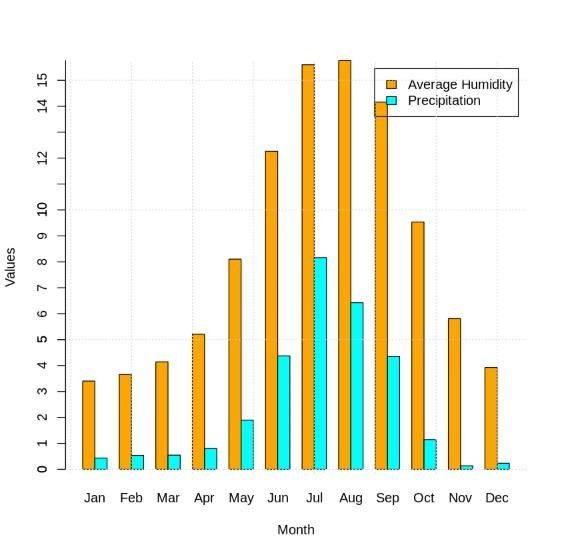
\includegraphics[width=0.6\textwidth]{figures/barchart3.jpg}
\caption{Comparing Monthly Averages: Humidity vs. Precipitation}
\label{fig:monthly_avg_bar}
\end{figure}

\paragraph{How to Interpret This Plot} Each pair of bars corresponds to a month:
\begin{itemize}
  \item Orange bar: Average humidity (\%)
  \item Cyan bar: Average precipitation (mm)
\end{itemize}

\paragraph{Interactive Questions:}
\begin{enumerate}
  \item In which month do humidity and precipitation both peak?
  \item Are there any months where humidity is high but precipitation is low?
  \item What might cause humidity to remain high even when there is little rainfall?
\end{enumerate}

\subsection*{Monthly Extremes: Hottest Month and Driest Month}

Climate extremes help us understand the variability and potential anomalies across the year. In this section, we identify:
\begin{itemize}
  \item The month with the highest average temperature.
  \item The month with the lowest average precipitation.
\end{itemize}

These extremes are valuable for seasonal planning, climate pattern analysis, and risk management.

\paragraph{Step-by-Step Approach}

We used the monthly summary data, already grouped by month, to identify these extremes.

\begin{verbatim}
highest_temp <- monthly_summary[which.max(monthly_summary$avg_temp), ]
lowest_temp <- monthly_summary[which.min(monthly_summary$avg_precip), ]

highest_temp
lowest_temp
\end{verbatim}

% Figure here----------------------------
\begin{figure}[h]
\centering
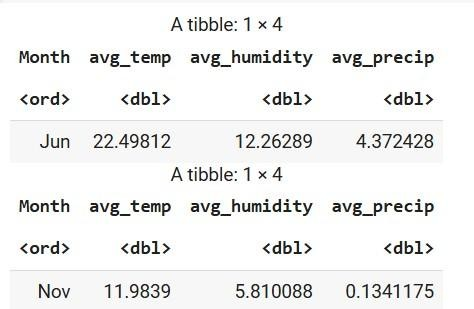
\includegraphics[width=0.5\textwidth]{figures/temp_highlow.jpg}
\caption{Month with Lowest and Highest Temperature}
\label{fig:extremes}
\end{figure}

\subsubsection*{Visualization Using ggplot2 and gridExtra}

The plots below visually highlight these extremes:  
Bar Plot for Temperature: Shows average monthly temperatures, with the hottest month labeled.  
Line Plot for Precipitation: Shows average monthly precipitation, with the driest month labeled.

\paragraph{R Code for Dual Plot Visualization:}

\begin{verbatim}
install.packages("gridExtra")
library(gridExtra)

p1 <- ggplot(monthly_summary, aes(x = as.factor(Month), y = avg_temp)) +
geom_bar(stat = "identity", fill = "red", alpha = 0.5) +
labs(title = "Monthly Temperature", x = "Month", 
y = "Temperature (°C)") +
geom_text(aes(label = ifelse(avg_temp == highest_temp$avg_temp,
paste("Max:", avg_temp, "°C"), "")),
vjust = -0.5, color = "black") +
theme_minimal()

p2 <- ggplot(monthly_summary, aes(x = as.factor(Month), y = avg_precip)) +
geom_line(group = 1) +
geom_point() +
labs(title = "Average Monthly Precipitation", x = "Month", 
y = "Precipitation") +
geom_text(aes(label = ifelse(avg_precip == lowest_temp$avg_precip,
paste("Min:", avg_precip, "°C"), "")),
vjust = -0.5, color = "black") +
theme_minimal()
grid.arrange(p1, p2, nrow = 1, ncol = 2)
\end{verbatim}

\begin{figure}[h]
\centering
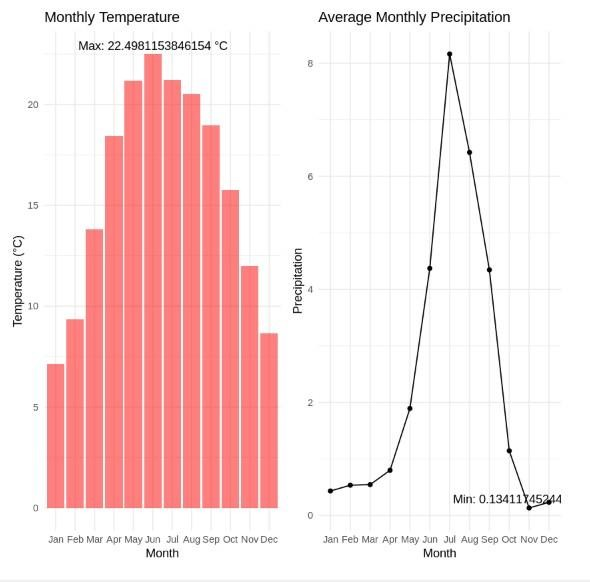
\includegraphics[width=0.5\textwidth]{figures/barchart1.jpg}
\caption{Bar Chart and Line Plot Showing Extreme Events}
\label{fig:dual_extremes}
\end{figure}

\paragraph{How to Interpret These Plots}
\begin{itemize}
  \item The left bar chart clearly marks the month with the highest average temperature.
  \item The right line chart pinpoints the month with the lowest average precipitation.
\end{itemize}

\paragraph{Questions to Explore:}
\begin{itemize}
  \item Does the hottest month align with the driest month?
  \item How do these extremes compare with seasonal expectations in your region?
  \item What implications might this have for agriculture or water resource planning?
\end{itemize}

\subsection*{Seasonal Insights}

\paragraph{Objective:} Identify climate patterns by season to understand how temperature, precipitation, and humidity vary across different times of the year.

\paragraph{Season Classification} To analyze seasonal trends, we categorized each month into one of four standard meteorological seasons:
\begin{itemize}
  \item Spring: March – May
  \item Summer: June – August
  \item Autumn: September – November
  \item Winter: December – February
\end{itemize}

\paragraph{The R code used for classification and aggregation:}

\begin{verbatim}
climate_data$Season <- case_when(
  climate_data$Month_Num %in% c(3,4,5) ~ "Spring",  # Mar-May
  climate_data$Month_Num %in% c(6,7,8) ~ "Summer",  # Jun-Aug
  climate_data$Month_Num %in% c(9,10,11) ~ "Autumn", # Sep-Nov
  climate_data$Month_Num %in% c(12,1,2) ~ "Winter"  # Dec-Feb
)

seasonal_avg <- climate_data %>%
  group_by(Season) %>%
  summarize(
    Avg_Temperature = mean(Temp_2m, na.rm = TRUE),
    Avg_Precipitation = mean(Precip, na.rm = TRUE),
    Avg_Humidity = mean(Humidity_2m, na.rm = TRUE)
  )
\end{verbatim}

\paragraph{Reshaping Data for Visualization}

To visualize all three variables in a single grouped bar chart, the dataset was converted from wide to long format:

\begin{verbatim}
seasonal_avg_long <- seasonal_avg %>%
  gather(key = "Variable", value = "Value", -Season)
\end{verbatim}

\paragraph{Visualization: Seasonal Climate Patterns}

\begin{verbatim}
ggplot(seasonal_avg_long, aes(x = Season, y = Value, fill = Variable)) +
geom_bar(stat = "identity", position = "dodge") +
labs(
title="Seasonal Climate Patterns: Temperature, Precipitation and Humidity",
x = "Season",
y = "Average Value",
fill = "Variable"
) +
theme_minimal()
\end{verbatim}

% Figure here-------------------------
\begin{figure}[h]
\centering
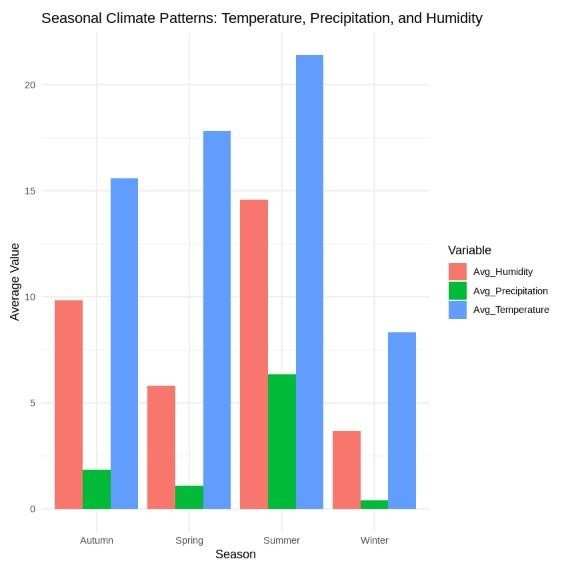
\includegraphics[width=0.5\textwidth]{figures/barchart.jpg}
\caption{Bar Chart Showing Seasonal Climate Pattern}
\end{figure}

\paragraph{Interpretation and Insights} This grouped bar chart shows the average temperature, precipitation, and humidity for each season. It allows for direct comparison across seasons and between variables.

For example, if summer shows high temperature but low humidity and precipitation, it may indicate a dry season.

\paragraph{Interactive Thought:}

Which season experiences the most rainfall? Is that also the most humid? How do these seasonal shifts align with regional agricultural activities or disaster preparedness plans?
\clearpage

